\chapter{Implementation}

\section{Module Overview}

The Smart Interview AI platform is implemented as a collection of interconnected modules. Figure~\ref{fig:modules} shows the high-level module decomposition.

\begin{figure}[H]
\centering
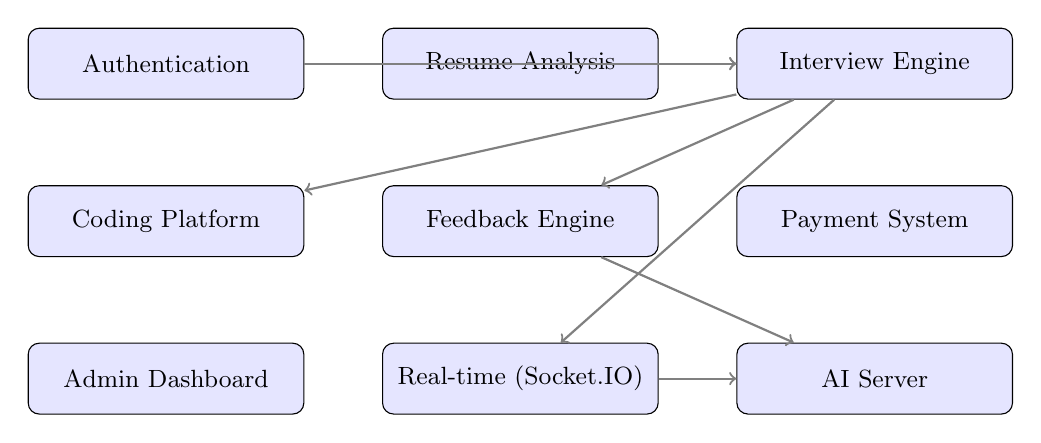
\begin{tikzpicture}[
  mod/.style={rectangle, draw, rounded corners, fill=blue!10, minimum width=3.5cm, minimum height=0.9cm, text centered, font=\small},
  arrow/.style={->, thick, gray}
]
\node[mod] (auth) at (0,0) {Authentication};
\node[mod] (resume) at (4.5,0) {Resume Analysis};
\node[mod] (interview) at (9,0) {Interview Engine};
\node[mod] (coding) at (0,-2) {Coding Platform};
\node[mod] (feedback) at (4.5,-2) {Feedback Engine};
\node[mod] (payment) at (9,-2) {Payment System};
\node[mod] (admin) at (0,-4) {Admin Dashboard};
\node[mod] (socket) at (4.5,-4) {Real-time (Socket.IO)};
\node[mod] (ai) at (9,-4) {AI Server};

\draw[arrow] (auth) -- (interview);
\draw[arrow] (resume) -- (interview);
\draw[arrow] (interview) -- (feedback);
\draw[arrow] (interview) -- (coding);
\draw[arrow] (interview) -- (socket);
\draw[arrow] (socket) -- (ai);
\draw[arrow] (feedback) -- (ai);
\end{tikzpicture}
\caption{Module Decomposition}
\label{fig:modules}
\end{figure}

\section{Authentication Module}

\subsection{Implementation Details}

The authentication system uses JSON Web Tokens (JWT) with a dual-token strategy:

\begin{itemize}
    \item \textbf{Access Token:} Short-lived (15 minutes), used for API authentication.
    \item \textbf{Refresh Token:} Long-lived (7 days), used to obtain new access tokens.
\end{itemize}

Passwords are hashed using bcrypt with a cost factor of 12. Account lockout is implemented after 5 consecutive failed login attempts, with a 2-hour lock duration.

\begin{lstlisting}[language=JavaScript, caption={JWT Token Generation}]
export function generateTokens(userId: string): AuthTokens {
  const accessToken = jwt.sign(
    { userId },
    process.env.JWT_ACCESS_SECRET!,
    { expiresIn: '15m' }
  );
  const refreshToken = jwt.sign(
    { userId },
    process.env.JWT_REFRESH_SECRET!,
    { expiresIn: '7d' }
  );
  return { accessToken, refreshToken };
}
\end{lstlisting}

\subsection{Security Measures}

\begin{itemize}
    \item Auth0 tokens are NOT accepted without signature verification (security fix applied).
    \item In production, database downtime returns HTTP 503 instead of bypassing authentication.
    \item All routes except \texttt{/api/auth/*} and \texttt{/api/health} require a valid JWT.
\end{itemize}

\section{Interview Engine}

\subsection{Question Generation}

Questions are generated using the Google Gemini 2.5 Flash model. The prompt is constructed dynamically based on:
\begin{itemize}
    \item Interview type (technical, behavioural, coding, system design, skill-based).
    \item Target role (e.g., ``Full Stack Developer'').
    \item Difficulty level (easy, medium, hard).
    \item Session duration (determines question count: min(5, duration/5)).
    \item Resume context (skills, projects, experience) if a resume is uploaded.
    \item Domain (for skill-based interviews, e.g., ``React'', ``DBMS'').
\end{itemize}

For coding interviews, the prompt enforces a strict JSON schema requiring \texttt{testCases}, \texttt{examples}, and \texttt{constraints} fields. A fallback question set is used only when Gemini is completely unavailable.

\subsection{Interview Flow}

Figure~\ref{fig:interviewflow} illustrates the complete interview session flow.

\begin{figure}[H]
\centering
\begin{tikzpicture}[
  step/.style={rectangle, draw, rounded corners, fill=green!10, minimum width=4cm, minimum height=0.8cm, text centered, font=\small},
  decision/.style={diamond, draw, fill=yellow!10, minimum width=2cm, minimum height=0.8cm, text centered, font=\tiny, aspect=2},
  arrow/.style={->, thick}
]
\node[step] (setup) at (0,0) {Interview Setup};
\node[step] (create) at (0,-1.5) {Create Interview (Gemini)};
\node[step] (start) at (0,-3) {Start Session};
\node[step] (question) at (0,-4.5) {Display Question};
\node[step] (answer) at (0,-6) {Candidate Answers};
\node[step] (submit) at (0,-7.5) {Submit Response};
\node[step] (analysis) at (4,-7.5) {Background AI Analysis};
\node[decision] (more) at (0,-9) {More Questions?};
\node[step] (end) at (0,-11) {End Interview};
\node[step] (feedback) at (0,-12.5) {Generate Feedback};

\draw[arrow] (setup) -- (create);
\draw[arrow] (create) -- (start);
\draw[arrow] (start) -- (question);
\draw[arrow] (question) -- (answer);
\draw[arrow] (answer) -- (submit);
\draw[arrow] (submit) -- (analysis);
\draw[arrow] (submit) -- (more);
\draw[arrow] (more) -- node[right, font=\tiny] {Yes} (question);
\draw[arrow] (more) -- node[right, font=\tiny] {No} (end);
\draw[arrow] (end) -- (feedback);
\end{tikzpicture}
\caption{Interview Session Flow}
\label{fig:interviewflow}
\end{figure}

\subsection{Response Submission and Analysis}

The response submission endpoint uses a fire-and-return pattern:
\begin{enumerate}
    \item Save the response to MongoDB immediately.
    \item Return HTTP 200 to the client instantly.
    \item Run Gemini analysis asynchronously in the background.
    \item Update content metrics in MongoDB when analysis completes.
\end{enumerate}

A critical bug was identified and fixed: if the user ends the interview before background analysis completes, the feedback page would show zero scores. The fix runs synchronous analysis on all responses during feedback generation if metrics are still zero.

\section{Coding Interview Module}

\subsection{Architecture}

The coding interview module consists of:
\begin{itemize}
    \item \textbf{Frontend:} Monaco Editor with language switching, test case display, and output console.
    \item \textbf{Backend:} Code execution service using the Piston API.
    \item \textbf{Test Harness:} Language-specific wrappers that parse multi-line inputs and call the user's function with correct arguments.
\end{itemize}

\subsection{Python Test Harness}

A key challenge was correctly passing arguments to user-defined functions. The test input format is multi-line (e.g., \texttt{[2,7,11,15]\textbackslash n9} for Two Sum), but users may name their function anything. The harness:

\begin{enumerate}
    \item Parses each input line using \texttt{json.loads} with \texttt{ast.literal\_eval} fallback.
    \item Detects the user's function using Python introspection.
    \item Expands arguments to match the function's parameter count.
    \item Tries multiple calling conventions with a fallback chain.
\end{enumerate}

\begin{lstlisting}[language=Python, caption={Python Argument Normalisation}]
def _expand_args(args, fn):
    n_params = _get_param_count(fn)
    # Already correct number of args
    if n_params is not None and len(args) == n_params:
        return args
    # Single dict: map keys to params
    if len(args) == 1 and isinstance(args[0], dict):
        payload = args[0]
        param_names = list(inspect.signature(fn).parameters.keys())
        if all(name in payload for name in param_names):
            return [payload[name] for name in param_names]
    # Single list with right number of items
    if len(args) == 1 and isinstance(args[0], (list, tuple)):
        inner = list(args[0])
        if n_params is not None and len(inner) == n_params:
            return inner
    return args
\end{lstlisting}

\subsection{Output Normalisation}

Test case comparison uses JSON normalisation to handle formatting differences:
\begin{lstlisting}[language=JavaScript, caption={Output Normalisation}]
private normalizeOutput(value: string): string {
  const trimmed = value.trim();
  try {
    return JSON.stringify(JSON.parse(trimmed));
  } catch {
    return trimmed.toLowerCase();
  }
}
\end{lstlisting}

\section{Resume Analysis Module}

\subsection{Upload Pipeline}

\begin{enumerate}
    \item User uploads PDF/DOC/DOCX via multipart form data.
    \item Multer stores the file in memory (no disk write).
    \item The file is uploaded to Cloudinary (with local fallback).
    \item The file buffer is sent to the Python AI server for parsing.
    \item Extracted data is stored in MongoDB.
\end{enumerate}

\subsection{ATS Scoring}

The ATS score is computed as:
\begin{equation}
\text{ATS Score} = 50 + \min(2 \times |\text{skills}|, 20) + \min(5 \times \text{experience}, 15) + \min(5 \times |\text{education}|, 10) + \min(2 \times |\text{certs}|, 5)
\end{equation}

\subsection{Download and View}

Resume files are served through the backend (not directly from Cloudinary) to keep storage URLs private. The backend fetches the file from Cloudinary using Axios with \texttt{responseType: 'stream'} and pipes it to the client response.

\section{Real-Time Communication}

Socket.IO is used for real-time features:
\begin{itemize}
    \item \textbf{Video frame analysis:} The frontend sends base64-encoded frames every 2 seconds; the backend forwards them to the Python AI server and emits results back.
    \item \textbf{Audio analysis:} Transcripts are sent for filler word detection and speech pattern analysis.
    \item \textbf{Interview status updates:} Question navigation, typing indicators, and session state changes.
\end{itemize}

\section{Deployment Architecture}

\begin{figure}[H]
\centering
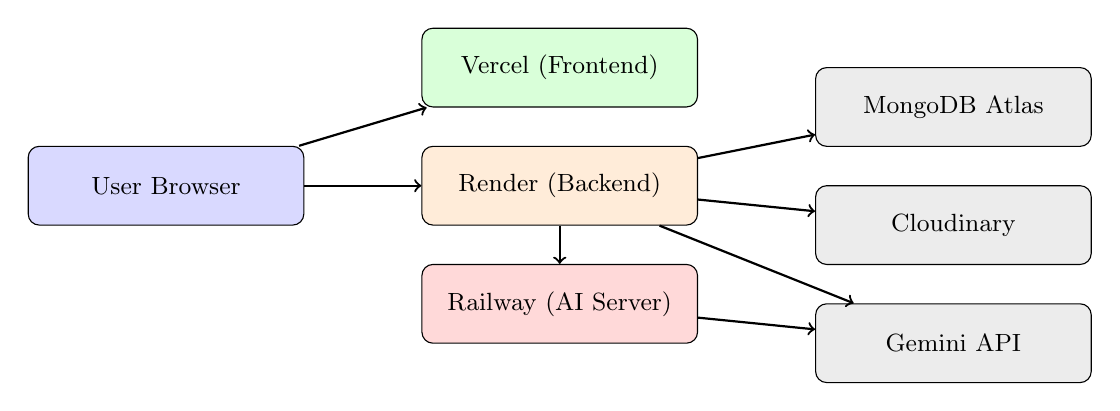
\begin{tikzpicture}[
  box/.style={rectangle, draw, rounded corners, minimum width=3.5cm, minimum height=1cm, text centered, font=\small},
  arrow/.style={->, thick}
]
\node[box, fill=blue!15] (user) at (0,0) {User Browser};
\node[box, fill=green!15] (vercel) at (5,1.5) {Vercel (Frontend)};
\node[box, fill=orange!15] (render) at (5,0) {Render (Backend)};
\node[box, fill=red!15] (railway) at (5,-1.5) {Railway (AI Server)};
\node[box, fill=gray!15] (atlas) at (10,1) {MongoDB Atlas};
\node[box, fill=gray!15] (cloudinary) at (10,-0.5) {Cloudinary};
\node[box, fill=gray!15] (gemini) at (10,-2) {Gemini API};

\draw[arrow] (user) -- (vercel);
\draw[arrow] (user) -- (render);
\draw[arrow] (render) -- (railway);
\draw[arrow] (render) -- (atlas);
\draw[arrow] (render) -- (cloudinary);
\draw[arrow] (render) -- (gemini);
\draw[arrow] (railway) -- (gemini);
\end{tikzpicture}
\caption{Production Deployment Architecture}
\label{fig:deployment}
\end{figure}

\subsection{Frontend Deployment (Vercel)}

\begin{itemize}
    \item Build command: \texttt{npm run build} (Vite).
    \item Output directory: \texttt{dist}.
    \item SPA routing: \texttt{vercel.json} rewrites all paths to \texttt{index.html}.
    \item Environment variable: \texttt{VITE\_API\_BASE\_URL} set to the Render backend URL.
\end{itemize}

\subsection{Backend Deployment (Render)}

\begin{itemize}
    \item Build command: \texttt{npm install \&\& npm run build} (TypeScript compilation).
    \item Start command: \texttt{npm start} (runs \texttt{node dist/server.js}).
    \item Root directory: \texttt{backend}.
    \item DNS override to Google (8.8.8.8) for MongoDB Atlas SRV resolution.
\end{itemize}

\newpage
